\documentclass[conference]{IEEEtran}
\IEEEoverridecommandlockouts
% The preceding line is only needed to identify funding in the first footnote. If that is unneeded, please comment it out.
\usepackage{cite}
\usepackage{amsmath,amssymb,amsfonts}
\usepackage[hidelinks]{hyperref}
\usepackage{algorithmic}
\usepackage{graphicx}
\usepackage{booktabs}
\usepackage{textcomp}
\usepackage{xcolor}
\def\BibTeX{{\rm B\kern-.05em{\sc i\kern-.025em b}\kern-.08em
    T\kern-.1667em\lower.7ex\hbox{E}\kern-.125emX}}
\begin{document}


\title{Composition of concrete and its influence on compressive strength\\
%{\footnotesize \textsuperscript{*}Note: Sub-titles are not captured in Xplore and
%should not be used}
%\thanks{Identify applicable funding agency here. If none, delete this.}
}

\author{\IEEEauthorblockN{Filipe P. de Farias}
\IEEEauthorblockA{\textit{Department of Teleinformatics Engineering} \\
\textit{Federal University of Ceará}\\
Fortaleza, Brazil \\
filipepfarias@fisica.ufc.br}
\and
\IEEEauthorblockN{Yvo J. M. Sales}
\IEEEauthorblockA{\textit{Department of Teleinformatics Engineering} \\
\textit{Federal University of Ceará}\\
Fortaleza, Brazil \\
yvo@gtel.ufc.br}
}

\maketitle

\begin{abstract}
The compressive strength of concrete impacts directly on its application. The difference between the concrete for columns or beams and the concrete for pavements is mainly due the compressive strength it is able to resist. In this work, we perform an unconditional and a class-conditional mono-variate analysis as well as unconditional bi-variate and multi-variate analysis of the UCI concrete composition database.
\end{abstract}

\begin{IEEEkeywords}
concrete, compresive, strength, machine, learning, pre-processing
\end{IEEEkeywords}

\section{Introduction}
A material formed by aggregates bonded together by a fluid material that hardens over time has been used by humans for construction since many years ago\cite{b3}. Nowadays this material is known as concrete and it's widely used in the construction field. The aggregates used in the concrete affect directly its compressive strength which highly impacts its applications. For instance, in general, the concrete for columns or beams needs to have a greater compressive strength than the one for pavement. On this paper, we carry out an statistical analysis on a dataset extracted from the UCI Machine Learning Repository (University of California, Irvine)\cite{b4} that collects information about the concentration of some aggregates used to form different types of concretes and their resulting compressive strenght. 

This work is divided as follows. {\color{red}A description of the data is given in Section \ref{data_description}. The Section \ref{data_analysis} brings an unconditional and a class-conditional mono-variate analysis as well as unconditional bi-variate and multi-variate analysis of the data. Finally, the conclusions and considerations are exposed in Section }\ref{conclusions}.

% This works tries to predict this compressive strength and to classify when the concrete is proper to be applied in structures.  In the UCI database the concrete is tested with different components concentrations and different curing time (ages). 

\section{Data description}\label{data_description}

The composition of each of the $N$ concrete samples is given by the concentrations (kg/m\textsuperscript{3}) of $D$ components: Cement, Blast Furnace Slag, Fly Ash, Water, Superplasticizer, Coarse Aggregate and Fine Aggregate. Each sample has its Age (day) and the measured Concrete compressive strength (MPa), as described in Table~\ref{data_description_table}.

\begin{table}[htp]
\caption{Data description}
\begin{center}
  \begin{tabular}{@{} clc @{}}
    \toprule
    Component & Description & Unit \\ 
    \midrule
    $D_1$ & Cement & kg/m\textsuperscript{3} \\ 
    $D_2$ & Blast Furnace Slag & kg/m\textsuperscript{3} \\ 
    $D_3$ & Fly Ash & kg/m\textsuperscript{3} \\ 
    $D_4$ & Water & kg/m\textsuperscript{3} \\ 
    $D_5$ & Superplasticizer & kg/m\textsuperscript{3} \\ 
    $D_6$ & Coarse Aggregate & kg/m\textsuperscript{3} \\ 
    $D_7$ & Fine Aggregate & kg/m\textsuperscript{3} \\ 
    $D_8$ & Age & days \\ 
    $Y$ & Compressive strength & MPa \\ 
	\midrule
    N & 1030 samples&  \\ 
    \bottomrule
  \end{tabular}
\end{center}
\label{data_description_table}
\end{table}%

The concrete was stratified into $L=3$ classes\cite{b1}. The concrete which is weak and not recommended for structures, the \emph{Non-standard}, was labeled with $L_1$ and has 295 samples in it. The concrete whose strength is in a range that can be applied to structures is classified as $L_2$, or \emph{Standard}, and has 525 samples. The high performance concrete $L_3$, \emph{High-strength} and has 210 samples.
The observations are the measured compressive strengths of each sample and, as the predictors $D_1 - D_7$, are continuous. The Age ($D_8$) of the concrete is extremely discrete. The output is the concrete strength 

\begin{figure}[htbp]
\centerline{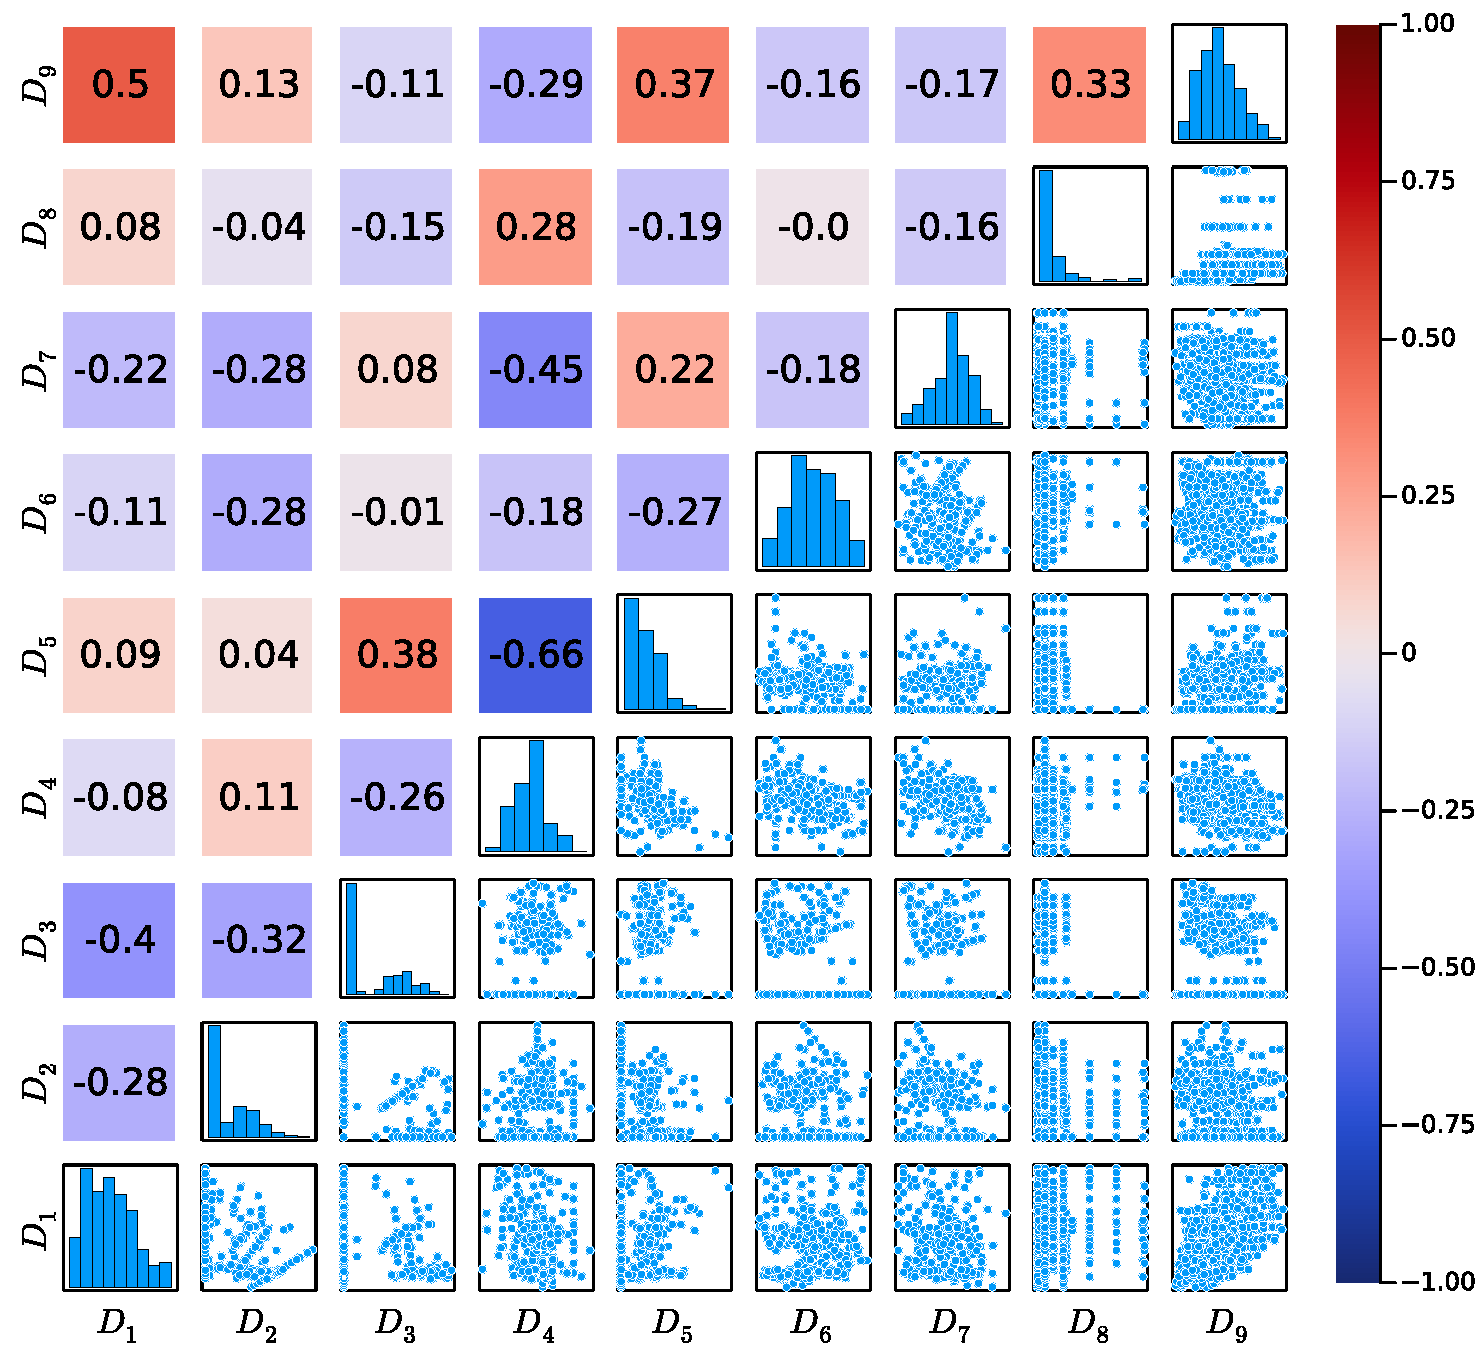
\includegraphics[width=\columnwidth]{../figures/correlation_predictors_outcomes}}
\caption{Pairwise scatter plot of each concrete component.}
\label{histogram_biplot}
\end{figure}

\section{Methods}\label{methods}

Regression models try to find relations between the \emph{independent variables} and the \emph{dependent variables}, which are named, respectively, predictors and outcomes in this work. These relations can occur in different forms. The simplest one is the linear relationship, which is when the curve predictors \textit{vs} outcomes, in the case that both are one-dimemsional, forms a simple line and, in the general case, a hyperplane. In what folows, we formluate the \emph{Linear regression}, which is a subclass of regressions dedicated to find a linear model to explain the relation between the predictors and the outcomes. 


\subsection{Linear regression}

This method tries to find the linear regression between the predictors and outcomes by fitting a line with linear coefficient $\beta_0$ and angular coefficient $\beta_1$, defined in Eq.~(\ref{eq:lm}), through the data. The fitting is done by minimising a cost function that can take different forms. Each cost function yields to different optimal parameters and two of them are described in the following, the \emph{Ordinary least squares} and \emph{L\textsubscript{2}-penalized least squares}. Regard the fact that $\beta_1$ can be a vector of the size such as the number of predictors in $X$. An interesting fact to observe is when the predictors correlates with the outcome, we can observe the error will be small. This is because the correlation evaluates linear variations between the variables as such as the linear regression.

\begin{align} \label{eq:lm}   
  Y &= \begin{bmatrix} 
        \beta_0 & \beta_1 
       \end{bmatrix} 
       \begin{bmatrix} 
        1 \\ X 
      \end{bmatrix} + \varepsilon
  %\\
  % \begin{bmatrix} \label{eq:estimated_betas}
  % \hat{\beta}_0 \\ \hat{\beta}_1
  % \end{bmatrix} &= \left( \begin{bmatrix}
  % 1 & X
  % \end{bmatrix}^\top
  % \begin{bmatrix}
  % 1 & X
  % \end{bmatrix} \right)^{-1}
  % \begin{bmatrix}
  % 1 & X
  % \end{bmatrix}^\top Y
\end{align} 

The \emph{Ordinary least squares} defines the cost function to find the optimal parameters for Eq.~(\ref{eq:lm}) as

\begin{equation}\label{eq:cf_ols}
  L(\mathbf{y}, \boldsymbol{\beta}) =\sum_{i=1}^{n}\left(y_{i}-\beta_{0}-\sum_{j=1}^{p} \beta_{j} x_{i j}\right)^{2},
\end{equation}
%
where $\mathbf{y} = [y_0, ..., y_p)]^T$ and $\boldsymbol{\beta} = [\beta_0, ..., \beta_p)]^T$.

The \emph{L\textsubscript{2}-penalized least squares} modifies Eq.~(\ref{eq:cf_ols}) adding a term that penalize large values of the parameters, yielding to

\begin{equation}
  L(\mathbf{y}, \boldsymbol{\beta}) = \sum_{i=1}^{n}\left(y_{i}-\beta_{0}-\sum_{j=1}^{p} \beta_{j} x_{i j}\right)^{2}+\lambda \sum_{j=1}^{p} \beta_{j}^{2},
\end{equation}
%
where $\mathbf{y} = [y_0, ..., y_p)]^T$, $\boldsymbol{\beta} = [\beta_0, ..., \beta_p)]^T$ and $\lambda$ is the penalization coefficient, which is a tuning parameter.

\emph{Partial least squares}

\section{Results}

\begin{figure}[htbp]
\centerline{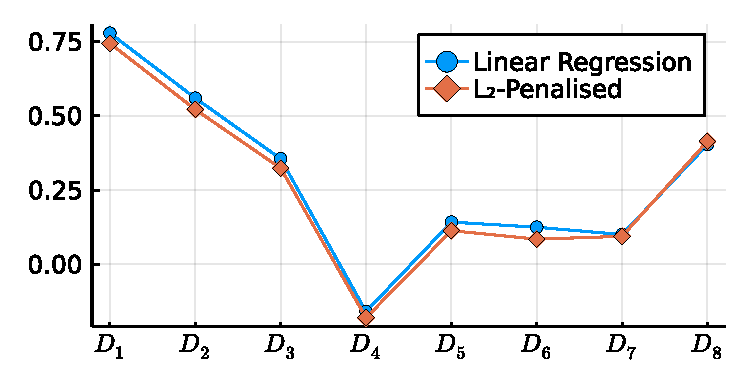
\includegraphics[width=\columnwidth]{../figures/fitted_params_70}}
\caption{Values of the weights of each predictor obtained after 30\%/70\% cross-validation strategy.}
%\label{histogram_biplot}
\end{figure}

\begin{figure}[htbp]
\centerline{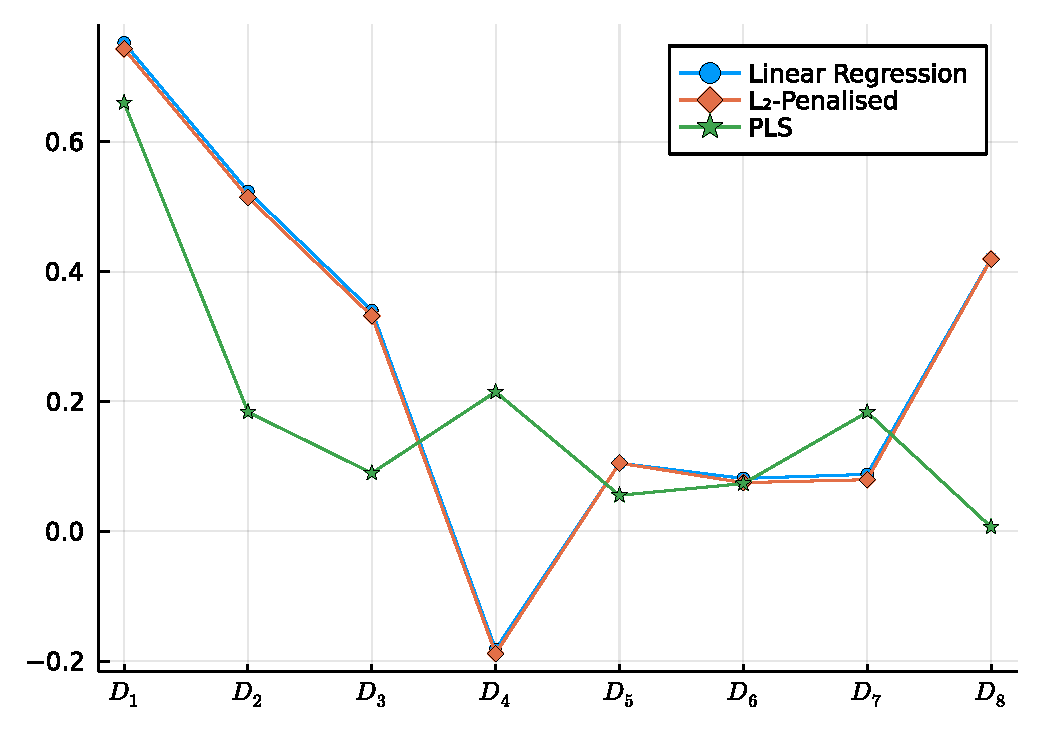
\includegraphics[width=\columnwidth]{../figures/fitted_params_kfolds}}
\caption{Values of the weights of each predictor obtained after $5$-fold cross-validation strategy.}%\label{histogram_biplot}
\end{figure}

\begin{table}[h!] 
\centering
  \caption{Ordinary Least Squares Regression Summary}
  \label{table:ols}
  \begin{tabular}{crr}
    \toprule
    {CV} & {RMSE} & {$R^2$} \\\hline
    70\% Train / 30\% Test & 0.614014 & 0.612271 \\
    1-st fold & 0.614187 & 0.634496 \\
    2-dn fold & 0.647336 & 0.597003 \\
    3-rd fold & 0.5952 & 0.599484 \\
    4-th fold & 0.686377 & 0.530463 \\
    5-th fold & \textbf{0.582266} & \textbf{0.661407} \\\bottomrule
  \end{tabular}
\end{table}


\begin{table}
\centering
  \caption{Ridge Regression}
  \begin{tabular}{crr}
    \toprule
    {CV} & {RMSE} & {$R^2$} \\\hline
    70\% Train / 30\% Test & 0.599004 & 0.640309 \\
    1-th fold & 0.613885 & 0.634857 \\
    2-th fold & 0.647344 & 0.596994 \\
    3-th fold & 0.594722 & 0.600127 \\
    4-th fold & 0.68599 & 0.530993 \\
    5-th fold & \textbf{0.582357} & \textbf{0.661302} \\\bottomrule
  \end{tabular}
\end{table}


\begin{table}[t]
\centering
  \caption{Partial Least Squares Regression Summary}
  \label{table:pls}
  \begin{tabular}{crr}
    \toprule
    {CV} & {RMSE} & {$R^2$} \\\hline
    70\% Train / 30\% Test & 0.599264 & 0.639996 \\
    1-st fold & 0.614106 & 0.634593 \\
    2-dn fold & 0.646593 & 0.597928 \\
    3-rd fold & 0.594709 & 0.600143 \\
    4-th fold & 0.6859 & 0.531116 \\
    5-th fold & \textbf{0.58221} & \textbf{0.661472} \\\bottomrule
  \end{tabular}
\end{table}


\section{Conclusion}\label{conclusions}

The database of concrete is not easy to analyse if there is no previous knowledge about the problem of the components mixture. In none of the analysis the data have been shown as separable on the initially determined classes. The next step is to try to perform regression to model the compressive strength itself before trying to classify the samples.

\begin{thebibliography}{00}
\bibitem{b1} ACI Manual of Concrete Practice 2000, Part 1: Materials and General Properties of Concrete.  American Concrete Institute.  Farmington Hills, MI.
\bibitem{b2} Tibshirani, Robert, et al. The Elements of  Statistical Learning:  Data Mining, Inference, and Prediction. Alemanha, Springer New York, 2009.
\bibitem{b3} Mindess, S., and Young, J.F. Concrete. Prentice-Hall, Inc., Englewood Cliffs, NJ, 1981.
\bibitem{b4} I-Cheng Yeh, "Modeling of strength of high performance concrete using artificial neural networks," Cement and Concrete Research, Vol. 28, No. 12, pp. 1797-1808 (1998)
\end{thebibliography}
\end{document}